\section{Methodology}
In this section, we explain our setup for determining Mamba's ability to learn
from context.
In our paper, we test 2 different models which attempt to use Mamba for its
in-context learning abilities against a variety of datasets, elaborated on
below.
\subsection{Data Format}
In plain English, the task we train is
\begin{quote}
    Each instance of our task is based on a \textbf{context image}, which
    is a photograph of a scene containing one or more words(e.x. photograph of a
    train station).
    We are also provided a set of AABBs surrounding each English word/token in
    the image(e.x. \verb|the|, \verb|,|).
    Our task is to predict the text associated with each word image.
\end{quote}
Since are trying to make Mamba, a sequence-to-sequence model, learn this task,
we propose an encodings of contexts as images.
As it stands, there already exists a method for transforming raster images into
sequences for Mamba, introduced in \cite{vmamba}.
We are trying to demonstrate improvement based on context, however, so we need
to add context to the sequences. We do this using 2 methods: Positional Encoding
and Text Injection

\subsubsection{Position Encoding}
An issue with our sequence transformation is that we destroy all 2-D positional
data.
Thus, before the sequence transformation, we append new channels to the image,
similar to the positional encodings mentioned in \cite{attention}.

\subsubsection{Text Injection}
\begin{figure}
    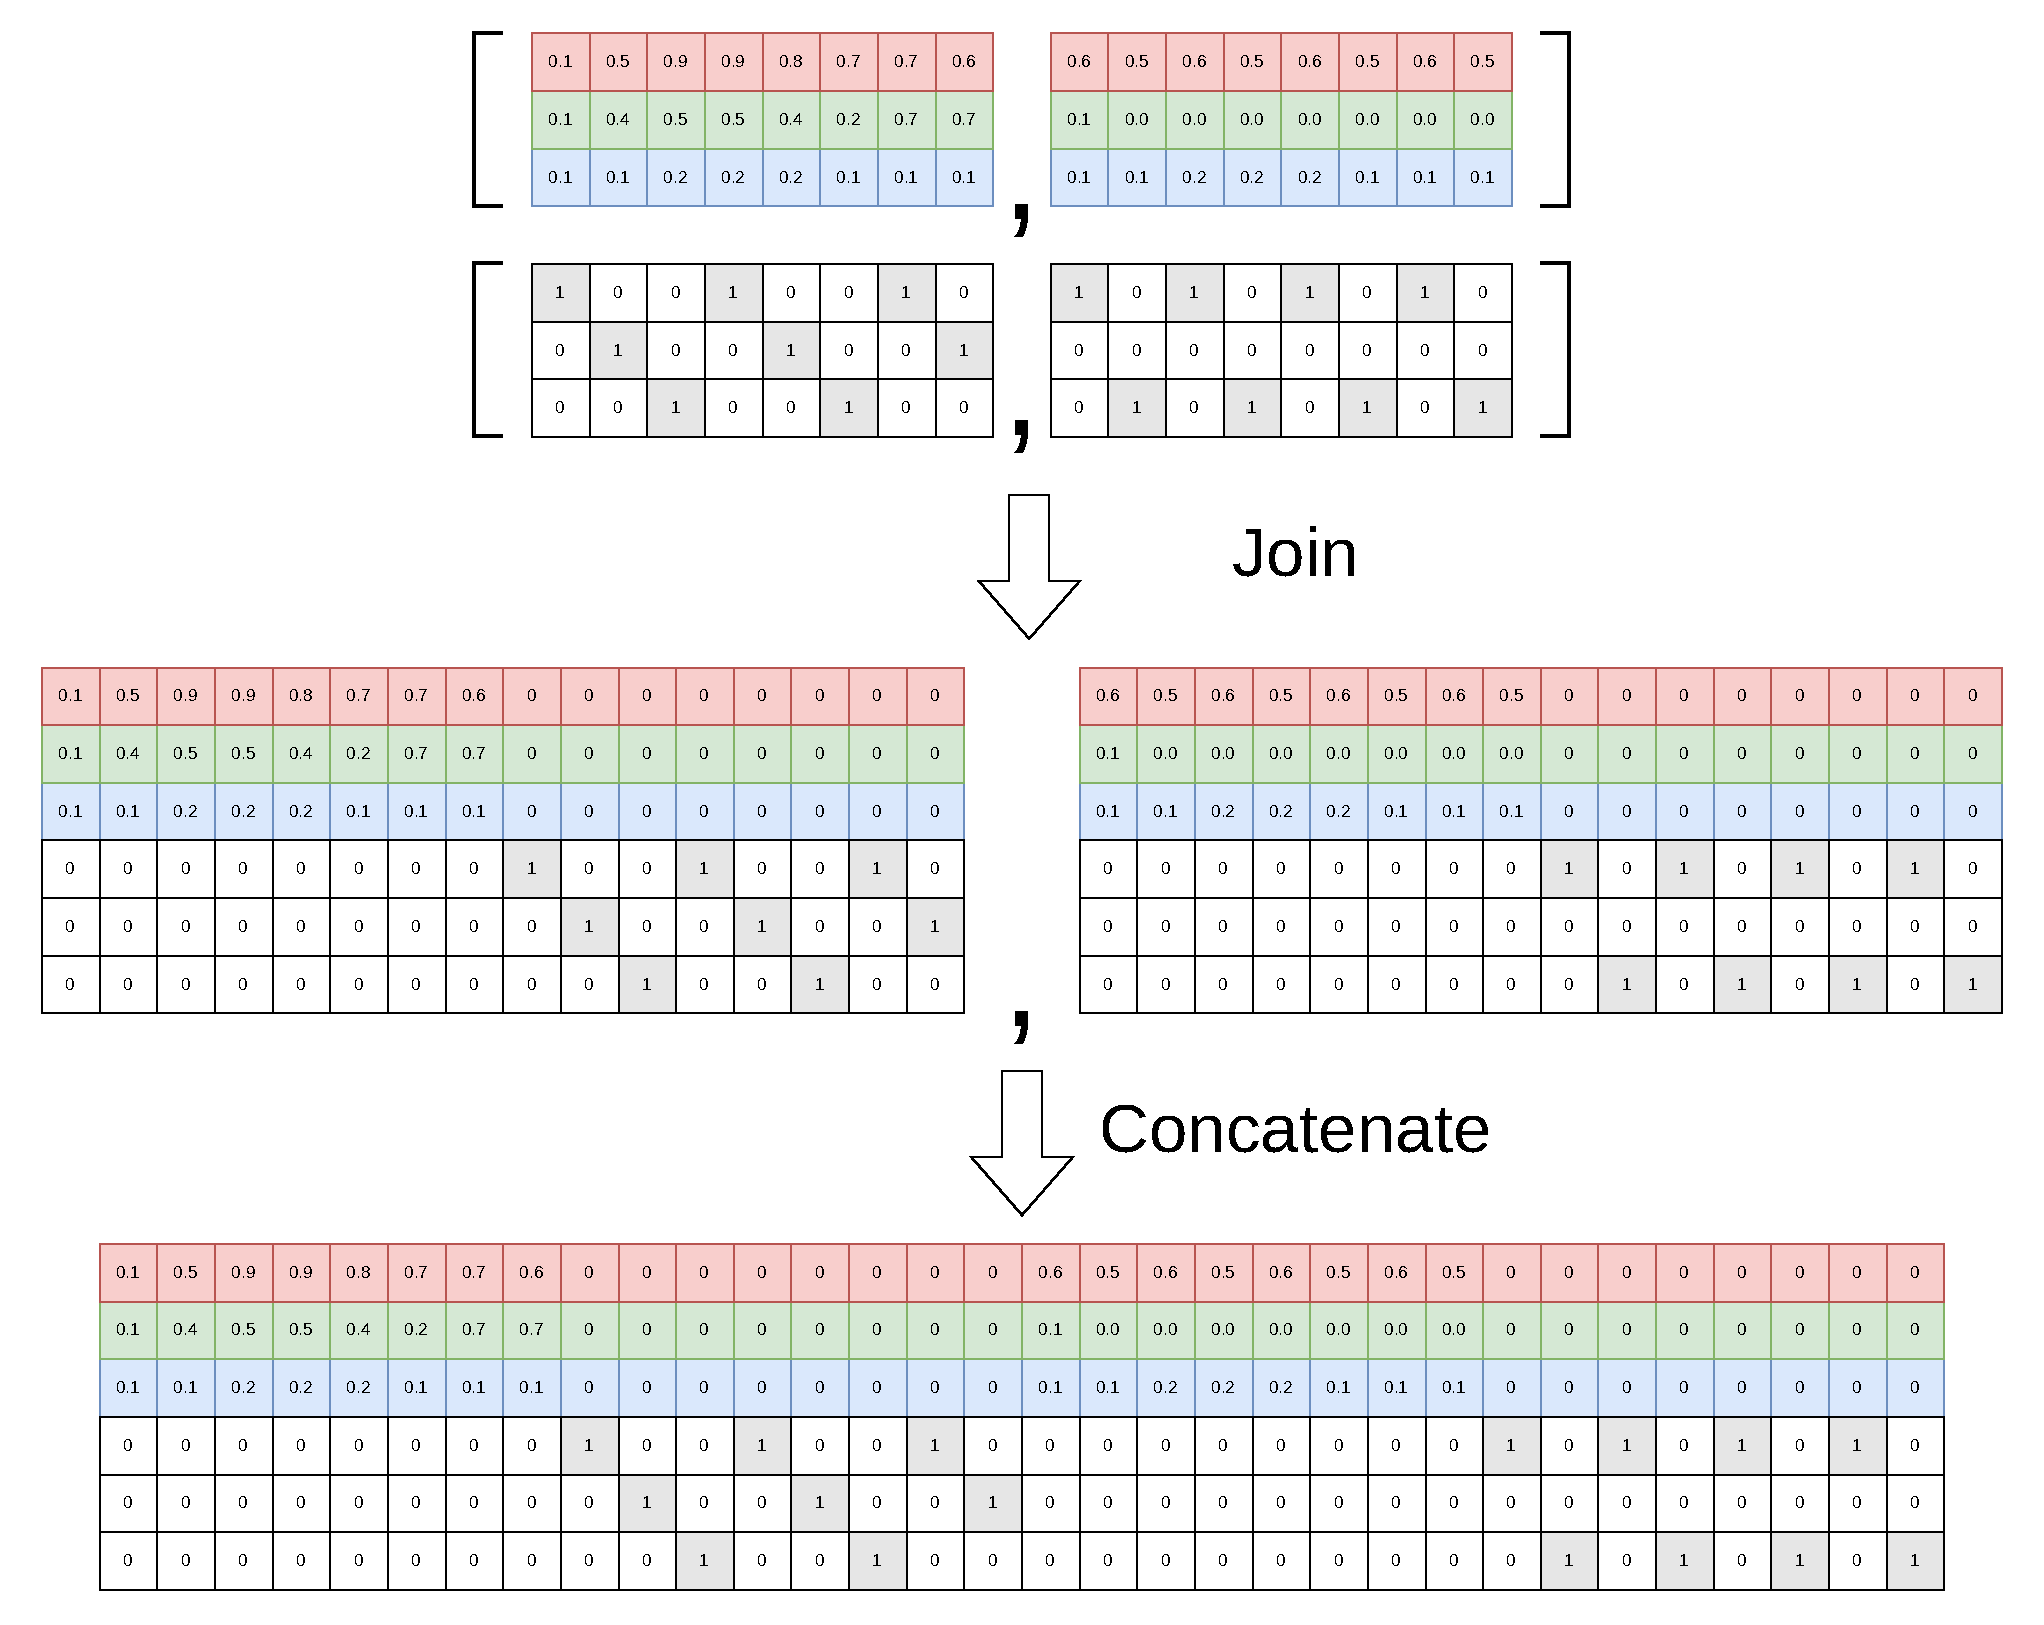
\includegraphics[width=\textwidth]{figures/in_context_encoding.pdf}
    \caption{In-Context Encoding}
    \label{incontextencoding}
\end{figure}

In order to supply context to the models, we encode our dataset using a scheme
that involves what we will call in-context encoding.
Before in-context encoding, all of the images within a context need to be
transformed into sequences.
We will call these sequences the image matrices, where each column corresponds
to a pixel in the image(with positional encodings and other per-pixel metadata)
Then, we encode the labels as one-hot tokens such that each label is represented
as a matrix of one-hot columns.
We now apply the in-context encoding transformation on these 2 lists of tensors.
First, we diagonally append the label tensors to the image sequence tensors such
that they are in separate channel spaces.
Then, we append all of the combined tensors lengthwise to get the final tensor.
This process is shown in Figure \ref{incontextencoding}.

With this encoding scheme, we assume that the data is being processed by an
auto-regressive model, where each output token is evaluated based on the
previous (correct) output tokens, and previous predictions in context.

We hypothesize that Mamba's ability to do in-context learning\cite{mamba} will
allow model architectures containing Mamba to perform well on in-context
image prediction.

\subsection{Mamba Stack}
The first model architecture that we test is a stack of Mamba layers. In our
previous testing, we found these to perform well on finite memorization tasks,
so we expect this model to do relatively well.

\subsection{Mamba With CNN}
Another model architecture we look at  they run CNN layers
parallel to Mamba layers.
\subsection{}
